\chapter{팽창하는 뉴턴 우주}

\lectureoverview{현대 우주론은 우주 자체를 물리계로 다루면서 시작된다. 큰 규모에서의 등방성과 균질성을 출발점으로 삼아 공변 격자를 도입하고, 그 운동을 하나의 척도 인자 \(a(t)\)로 나타낸다. 뉴턴의 껍질 정리는 중력 다체 문제를 \(a(t)\)에 관한 방정식으로 바꾸어 준다. 에너지 보존은 재수축하는 우주, 임계 우주, 영원히 팽창하는 우주를 구분하며, 임계인 물질 지배 우주에서는 최초의 프리드만 방정식과 법칙 \(a(t)\propto t^{2/3}\)을 얻는다.}

\section{우주론이 물리학이 된 때}

우주론이라는 주제는 오래되었지만, 정량적 우주론은 역사가 짧다. 여기서는 그리스 시대부터 시작할 필요가 없다. 유용한 역사적 출발점은 20세기 중반에 허블이 우주의 팽창을 발견한 일과, 그 뒤 약 3켈빈의 마이크로파 배경 복사가 뜨거웠던 초기 우주의 잔재임을 알아낸 일이다.

측정이 정밀해지기 전에는 천문학의 상당 부분이 필연적으로 자연사와 비슷했다. 특이한 별을 발견하고, 독특한 은하를 분류하고, 측정할 수 있는 것을 측정한 뒤 천체 목록을 만들었다. 그 천체들은 분명 물리계였다. 각운동량을 지녔고, 화학 원소를 포함했으며, 역학 법칙을 따랐다. 결정적인 변화는 \emph{우주 전체}를 관측과 대조할 수 있을 만큼 정확한 방정식이 지배하는 하나의 물리계로 다루기 시작한 것이었다.

여기서 다룰 주제가 바로 그것이다. 우주의 구성 요소를 열거하는 데 그치지 않고, 우주의 변수와 운동, 그리고 동역학 법칙을 묻겠다. 방정식은 우주론 뒤에 덧붙이는 장식이 아니다. 방정식은 우주를 물리학의 문제로 다루게 해 주는 수단이다.

역사적으로 팽창 우주는 일반 상대성 이론의 언어로 이해되었다. 그러나 논리적으로 보면 최초의 논증 상당 부분은 뉴턴 역학에 속한다. 큰 규모의 올바른 운동을 추측한 17세기 물리학자라면 놀랄 만큼 훌륭한 모형을 유도할 수 있었을 것이다. 뉴턴 역학으로 시작하는 이유는 상대성 이론을 대체하려는 것이 아니라, 상대성 이론이 나중에 기하학적으로 재구성하는 역학을 드러내려는 것이다.

\section{등방성, 균질성, 우주론적 원리}

첫 단계는 관측이다. 충분히 큰 규모에서 우주는 대략 \emph{등방적}이다. 하늘의 여러 영역에 대해 평균을 내고 우리은하의 전경 너머를 보면, 어느 방향에서나 거의 비슷하게 보인다. 이것은 우주가 정확히 균일하다는 뜻이 아니다. 가까운 별을 직접 보는 것과 텅 빈 영역을 보는 것은 다르며, 물질 분포에는 실제 구조가 있다. 등방성이란 큰 규모에서 평균을 낸 진술이다.

균질성은 이와 다른 진술이다. 평균을 낸 우주가 장소에 따라 같다는 뜻이다. 여러 은하 너머에 있는 관측자도 같은 방식으로 큰 규모의 평균을 내면, 우리가 보는 것과 대략 같은 종류의 우주를 보아야 한다.

첫 번째 근사에서는 은하를 질량점으로 간단히 다룰 수 있다. 관측 가능한 우주에는 대략 \begin{equation}
N_{\rm gal}\sim 10^{11}
\end{equation}개의 은하가 있고, 각 은하에는 별이 대략 \(10^{11}\)개 있다. 따라서 별은 약 \(10^{22}\)개다. 별 하나당 행성이 열 개라고 매우 거칠게 자릿수만 추정하면 행성은 \(10^{23}\)개에 이르는데, 재미있게도 행성의 몰수에 가까운 수다. 이 수치 추정은 동역학의 일부는 아니지만, 이상화하는 계의 규모를 가늠하게 해 준다.

\begin{classroomqa}\classquestion{관측 가능한 우주에는 은하가 대략 몇 개나 있을까요?}\lecturerresponse{약 천억 개, 즉 \(10^{11}\)개입니다. 은하 하나에 별이 대략 \(10^{11}\)개 있다고 보면, 관측 가능한 우주의 별은 약 \(10^{22}\)개입니다. 아래 계산에서는 은하 하나를 질량점 하나로 바꾸어 다루지만, 이 규모 추정은 염두에 둘 만합니다. \lecturetimestamp{00:06:08--00:07:05}}\end{classroomqa}

우리 주변의 등방성으로부터 왜 균질성을 추론할 수 있을까? 등방적이지만 \emph{균질하지는 않은} 분포를 생각해 보자. 밀도는 방향과 무관하면서 우리로부터의 거리에 따라 달라져야 한다. 사실상 우리 위치를 중심으로 한 동심원 껍질 구조가 되는 셈이다. 공통 중심에서 벗어난 관측자는 더는 등방성을 보지 못할 것이다. 따라서 두 가지 가능성이 있다: \begin{enumerate}\item 우리가 우주가 우리를 중심으로 배열된 특별한 중심에 있다.\item 큰 규모의 분포가 대략 균질하여, 우주 안의 어떤 지점도 특별하지 않다.\end{enumerate}두 번째 가능성이 더 간명하다. 등방성에 더해 우리 자신에게 우주론적 특권 위치를 부여하지 않으면 균질성에 이른다.

\begin{classroomqa}\classquestion{등방적이지만 균질하지 않은 분포는 어떤 모양일 수 있나요?}\lecturerresponse{분포는 우리로부터의 거리에만 의존해 변할 수 있으며, 우리 위치를 중심으로 한 껍질 모양의 패턴을 이룰 것입니다. 관측자가 그 중심에서 벗어나면 패턴은 등방성을 잃습니다. 따라서 우리 위치가 특별하지 않다면 등방성은 균질성을 가리킵니다. \lecturetimestamp{00:07:06--00:08:54}}\end{classroomqa}

이 두 가정을 합친 것을 \emph{우주론적 원리}라고 한다. 충분히 큰 규모에서 우주는 공간적으로 균질하고 등방적이라는 원리다. 이를 원리라고 부른다고 해서 증명되는 것은 아니다. 역사적으로 우주론자들은 관측이 강한 근거를 제공하기 전에 이 가정을 채택했다. 이 가정의 지위는 경험적 성공에서 나온다.

균질성도 정확한 성질은 아니다. 은하들은 은하단과 초은하단을 이루며, 관측 가능한 하늘의 아주 큰 부분에 걸친 구조에 대한 논의도 오래전부터 이어져 왔다. 적절한 주장은 평균을 내는 영역이 충분히 크면 요동이 평균화된다는 것이다---이 입문 논의에서는 수억 광년에서 대략 십억 광년 규모다. 관측에 따라 그 규모는 정밀하게 조정할 수 있다. 국소 구조가 기술을 지배하지 않을 때까지 거친 규모로 평균을 내는 것이 방법이다.

\begin{classroomqa}\audiencequestion{우주 마이크로파 배경 복사의 균일성은 우주론적 원리의 근거가 되나요?}\lecturerresponse{그렇다. 우주론적 원리는 강한 관측 근거가 나오기 전에 제안되었지만, 마이크로파 배경 복사는 나중에 초기 우주가 놀라울 만큼 매끄러웠음을 보여 주었다. 은하와 은하단은 그 매끄러운 상태에서 작은 편차가 자라 생겼다. 그것들이 큰 규모의 근거를 지우지는 않는다. \lecturetimestamp{00:10:53--00:11:43}}\end{classroomqa}

\section{은하와 함께 움직이는 격자}

관측적 근사를 선택하고 나면 변수를 정해야 한다. “물리 문제를 정식화하는 첫 단계는 무엇인가?”라는 질문에 교실에서 흔히 하는 답은 변수를 아는 것이고, 전통적인 답은 연필을 뾰족하게 깎는 것이다. 여기서 중요한 변수는 좌표를 잘 선택하면 찾을 수 있다.

\(x,y,z\)라는 표지가 붙은 3차원 격자를 생각해 보자. 이 표지들은 미터 단위로 측정한 거리가 아니라 좌표값이다. 작은 고유 운동을 평균 내어 없앤 뒤 각 은하가 격자의 고정된 지점에 머물도록 격자를 정하자. 그러면 은하들은 \emph{공변}한다.

은하들이 무작위로 움직인다면 이런 선택은 쓸모가 없을 것이다. 그러나 관측은 큰 규모에서 일관된 운동을 보여 준다. 이웃한 격자 셀은 팽창하거나 수축할 수 있지만, 그 팽창이나 수축은 어디서나 똑같이 일어난다. 따라서 모든 물리적 거리는 시간에 따라 변하는 공통 척도와 고정된 좌표 간격의 곱으로 쓸 수 있다.

두 은하 \(A\)와 \(B\) 사이에서, \begin{equation}
\begin{aligned}
d_{AB}(t)&=a(t)\,\Delta\chi_{AB},\\
\Delta\chi_{AB}
&=\sqrt{(x_A-x_B)^2+(y_A-y_B)^2+(z_A-z_B)^2}.
\end{aligned}
\label{eq:c01-physical-distance}
\end{equation}\(x\)좌표에서만 차이가 난다면 다음과 같이 간단해진다. \begin{equation}
d_{AB}(t)=a(t)\,\Delta x_{AB}.
\end{equation}\(a(t)\) 함수가 \emph{척도 인자}다. 절대적인 정규화는 관례에 불과하다. 모든 공변 좌표에 상수를 곱하고 \(a\)를 같은 상수로 나누어도 물리적 거리는 변하지 않는다. \(a(t_2)/a(t_1)\) 같은 비와 \(a\)로 나눈 도함수가 물리적 정보를 담는다.

방정식~\eqref{eq:c01-physical-distance}을 미분하자. 공변 간격은 고정되어 있으므로 \begin{equation}
v_{AB}=\dot a\sqrt{(\Delta x)^2+(\Delta y)^2+(\Delta z)^2}.
\end{equation}물리적 거리로 나누면 다음을 얻는다. \begin{equation}
\frac{v_{AB}}{d_{AB}}=\frac{\dot a}{a}\equiv H(t),
\label{eq:c01-hubble-parameter}
\end{equation}즉 \begin{equation}
\boxed{v_{AB}=H(t)d_{AB}.}
\label{eq:c01-hubble-law}
\end{equation}이상적인 균질 유동에서 성립하는 허블 법칙이다.

“허블 상수”라는 이름은 오해를 부를 수 있다. 한 우주 시각에서 \(H\)의 값은 균질 모형의 모든 장소에서 같지만, \(H(t)\)는 일반적으로 시간에 따라 변한다. 공간적으로 보편적이라는 말은 시간에 따라 일정하다는 뜻이 아니다.

\begin{classroomqa}\audiencequestion{모든 거리를 공통된 \(a(t)\)와 고정된 좌표 간격의 곱으로 쓴 순간, 이미 허블 법칙을 가정한 것인가요?}\lecturerresponse{이 가정은 분명 허블의 관측에서 동기를 얻었다. 일관된 후퇴의 증거가 없었다면 이렇게 설정하지 않았을 것이다. 이 설정의 가치는 그 증거를 체계화하는 데 있다. 은하마다 독립된 속도를 주는 대신, 팽창하는 하나의 격자로 기술한다. 이 기술을 채택하면 미분을 통해 비례 관계 \(v=Hd\)가 따라 나온다. \lecturetimestamp{00:24:20--00:25:33}}\end{classroomqa}

같은 운동은 말로 두 가지 방식으로 기술할 수 있다. 은하들이 공간을 가로질러 서로 멀어진다고 할 수도 있고, 은하들은 고정된 공변 위치에 머무는 가운데 격자---즉 그 사이의 물리적 공간---가 팽창한다고 할 수도 있다. 이 단계에서는 같은 수학을 표현하는 두 좌표 기술이다. 일반 상대성 이론에서는 팽창하는 공간이라는 표현이 특히 자연스러워지지만, 모든 시각에 같은 물리적 간격을 부여하는 두 기술은 관측으로 구별할 수 없다.

\section{공변 셀에서 질량을 계산하기}

중력을 도입하기 전에 질량을 따져 보자. 좌표 부피가 \begin{equation}
\Delta V_{\rm com}=\Delta x\,\Delta y\,\Delta z.
\end{equation}인 작은 좌표 셀을 생각하자. 국소 요동을 평균낼 수 있도록 은하를 많이 포함할 만큼은 커야 한다. \(\nu\)를 공변 좌표 부피 단위당 질량이라고 하자. 셀 안의 질량은 \begin{equation}
\Delta M=\nu\,\Delta x\,\Delta y\,\Delta z.
\label{eq:c01-comoving-mass}
\end{equation}이다. 셀은 물질과 함께 움직이므로 이상적인 유동에서 경계를 넘어가는 은하는 없고, \(\Delta M\)는 일정하다.

물리적 변의 길이는 좌표 변의 길이보다 \(a(t)\)배 길다. 따라서 물리적 부피는 \begin{equation}
\Delta V_{\rm phys}=a^3(t)\,\Delta x\,\Delta y\,\Delta z.
\end{equation}이다. 물리적 질량 밀도는 \begin{equation}
\boxed{\rho(t)=\frac{\Delta M}{\Delta V_{\rm phys}}=\frac{\nu}{a^3(t)}.}
\label{eq:c01-density-dilution}
\end{equation}이다. 압력이 없는 물질은 팽창에 따라 \(a^{-3}\)만큼 희석되고, 같은 법칙에 따라 수축하면 밀도가 높아진다.

여기까지는 동역학에 관한 가정을 하지 않았다. 유클리드 기하학과 운동학적 가정, 공변 셀에서의 질량 보존을 사용했다. 이제 중력을 도입한다.

\section{이제 뉴턴 역학을 도입하자}

무한히 균일한 물질 분포는 한쪽에서의 인력이 다른 쪽에서의 인력과 상쇄되므로 정지해 있을 것이라는 생각은 그럴듯하지만 틀렸다. 이런 비형식적인 상쇄로는 상대 가속도에 대한 일관된 방정식을 세울 수 없다. 뉴턴의 껍질 정리가 힘을 올바르게 정리해 준다.

아무 은하나 원점 \(O\)으로 선택하고, 고정된 공변 반지름 \(A\)에 있는 은하를 생각하자. \begin{equation}
R=\sqrt{x^2+y^2+z^2}.
\end{equation}이 은하의 물리적 반지름, 반지름 방향 속도, 반지름 방향 가속도는 다음과 같다. \begin{equation}
d=aR,
\qquad
\dot d=\dot a R,
\qquad
\ddot d=\ddot a R.
\label{eq:c01-radial-kinematics}
\end{equation}

\begin{figure}[ht]\centering
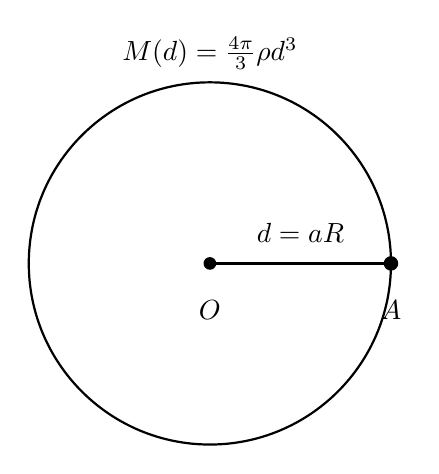
\begin{tikzpicture}[scale=1.15]
\draw[thick] (0,0) circle (2);
\fill (0,0) circle (0.07);
\fill (2,0) circle (0.08);
\draw[thick] (0,0) -- (2,0);
\draw (1,0.12) node[above] {\(d=aR\)};
\draw (0,-0.3) node[below] {\(O\)};
\draw (2,-0.3) node[below] {\(A\)};
\draw (0,2.32) node {\(M(d)=\frac{4\pi}{3}\rho d^3\)};
\end{tikzpicture}\caption{뉴턴 역학으로의 환원. 은하 \(A\)의 가속도를 구할 때 바깥쪽 껍질들의 힘은 상쇄되고, 반지름 \(d\) 안쪽의 질량은 \(O\)에 집중된 것처럼 작용한다.}\label{fig:c01-newton-sphere}\end{figure}

구대칭 질량 분포에서 \(A\)을 지나는 구면 바깥의 물질이 가하는 알짜 힘은 0이다. 내부 물질은 중심에 집중된 것처럼 작용한다. 둘러싸인 질량은 \begin{equation}
M(d)=\frac{4\pi}{3}\rho d^3.
\label{eq:c01-enclosed-mass}
\end{equation}이다. 그러면 뉴턴의 역제곱 법칙에 따라 \(A\)의 가속도는 다음과 같다. \begin{equation}
\ddot d=-\frac{GM(d)}{d^2}.
\end{equation}방정식~\eqref{eq:c01-radial-kinematics}을 사용하면 \begin{align}
\ddot a R
&=-\frac{G}{d^2}\left(\frac{4\pi}{3}\rho d^3\right) \\
&=-\frac{4\pi G}{3}\rho d \\
&=-\frac{4\pi G}{3}\rho aR.
\end{align}공변 반지름이 소거되어 \begin{equation}
\boxed{\frac{\ddot a}{a}=-\frac{4\pi G}{3}\rho.}
\label{eq:c01-acceleration}
\end{equation}을 얻는다. 이 소거가 일관성 검증이다. \(R\) 값과 관계없이 모든 공변 은하는 같은 척도 인자에 대해 같은 방정식을 따른다.

방정식~\eqref{eq:c01-density-dilution}을 대입하면 서로 동등한 두 형태를 얻는다. \begin{equation}
\frac{\ddot a}{a}=-\frac{4\pi G\nu}{3a^3},
\qquad
\ddot a=-\frac{4\pi G\nu}{3a^2}.
\label{eq:c01-acceleration-nu}
\end{equation}첫째 형태는 분율 가속도를 나타내고, 둘째 형태는 \(\ddot a\)를 분리해 보여 준다. \(a\)를 좌변에 두는 것은 관례일 뿐 물리학을 바꾸지 않는다.

\begin{classroomqa}\audiencequestion{원점은 임의로 골랐는데 계산에서 모든 힘은 그 원점을 향합니다. 원점을 다르게 잡아도 어떻게 같은 우주를 얻을 수 있나요?}\lecturerresponse{이 방정식은 상대 운동에 관한 것이다. 다른 은하를 중심으로 계산을 반복해도 균질성 때문에 둘러싸인 질량이 물리적 반지름에만 의존하므로 같은 방정식을 얻는다. 첫 원점에 대한 힘을 그대로 유지한 채 다른 은하에 붙은 가속 좌표계로 변환한다면, 그에 해당하는 관성력도 포함해야 한다. 중심 정지 좌표계를 택하면 그 추가 계산을 피할 수 있을 뿐이다. 불변인 결과는 특정 중심이 아니라 방정식~\eqref{eq:c01-acceleration}이다. \lecturetimestamp{00:43:56--00:46:58}}\end{classroomqa}

\begin{classroomqa}\audiencequestion{공변 질량 밀도 \(\nu\)가 장소에 따라 달라져도 결과가 성립하나요?}\lecturerresponse{이 한 함수로 된 형태로는 성립하지 않는다. 깔끔한 소거는 모든 곳에서 \(M\propto d^3\)가 같은 비례 관계를 따르는 데 달려 있다. 평균 규모를 가로질러 \(\nu\)가 눈에 띄게 변한다면 지역마다 서로 다른 동역학이 필요하고, 하나의 균질한 척도 인자로는 더 이상 기술할 수 없다. 균질성은 핵심적인 역할을 한다. \lecturetimestamp{00:47:05--00:47:51}}\end{classroomqa}

\begin{classroomqa}\audiencequestion{왜 \(\ddot a/a\)로 쓰고 인자 \(a\)를 우변으로 옮기지 않나요?}\lecturerresponse{두 형태 모두 옳다. 우주론에서는 관례적으로 분율 가속도 \(\ddot a/a\)를 쓴다. 부분적으로는 분율 팽창률 \(H=\dot a/a\)과 바로 비교할 수 있기 때문이다. 양변에 \(a\)를 곱하면 동일한 미분 방정식이 된다. \lecturetimestamp{00:50:36--00:51:29}}\end{classroomqa}

방정식~\eqref{eq:c01-acceleration}은 보통 물질로 채워진 정적인 균질 뉴턴 우주가 불가능함을 즉시 보여 준다. 정적인 척도 인자라면 \(\ddot a=0\)이어야 하지만, 양의 밀도에서는 우변이 음수다. 그렇다고 우주가 팽창하는지 수축하는지를 \emph{아직} 알려 주는 것은 아니다. 가속도의 부호만 알려 준다.

\section{음의 가속도는 수축을 뜻하지 않는다}

속도와 가속도의 차이는 기초적이지만 결정적이다. 아우토반에서 앞쪽으로 달리는 페라리는 속도가 양수인 채 제동하면서 음의 가속도를 가질 수 있다. 마찬가지로 우주도 \begin{equation}
\dot a>0,
\qquad
\ddot a<0:
\end{equation}일 수 있다. 즉 팽창하지만 팽창 속도는 줄어든다.

운동이 결국 역전되는지 판단하려면 우주론 문제를 지구 중력장에서 반지름 방향으로 움직이는 시험 입자와 비교하자. 이제 \(x\)는 중심 질량 \(M\)에서 입자까지의 물리적 거리를 뜻하며, 앞서 나온 공변 좌표와는 관계가 없다. 뉴턴 방정식은 \begin{equation}
\ddot x=-\frac{GM}{x^2}.
\label{eq:c01-particle-force}
\end{equation}이다. 가속도는 항상 안쪽을 향한다. 하지만 바깥쪽으로 던진 입자는 오랫동안, 또는 영원히 바깥쪽으로 계속 움직일 수 있다. 이미 안쪽으로 움직이는 입자는 속도가 점점 더 음수가 된다. 힘 법칙만으로는 어떤 운동이 일어날지 결정되지 않는다. 초기 조건이 결정한다.

\begin{classroomqa}\audiencequestion{\(\ddot a<0\)는 우주가 수축 중이라는 뜻인가요?}\lecturerresponse{아니다. 수축은 \(\dot a<0\)을 뜻한다. 음의 \(\ddot a\)는 \(\dot a\)가 시간에 따라 감소한다는 뜻일 뿐이다. \(\dot a\)가 처음에 양수라면 중력은 팽창을 늦춘다. 그것이 0에 이르는지는 초기 팽창 속도에 달려 있다. 바깥으로 움직이는 발사체의 운명이 탈출 속도보다 느린지 빠른지에 달린 것과 정확히 같다. \lecturetimestamp{00:51:30--00:56:18}}\end{classroomqa}

\begin{figure}[ht]\centering
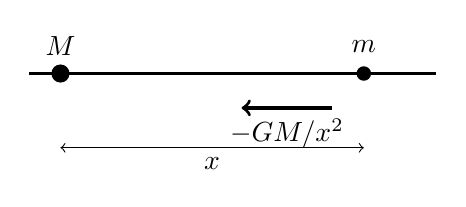
\begin{tikzpicture}[scale=1.15]
\fill (0,0) circle (0.1);
\draw (0,0.3) node {\(M\)};
\draw[thick] (-0.35,0) -- (4.15,0);
\fill (3.35,0) circle (0.08);
\draw (3.35,0.3) node {\(m\)};
\draw[->,very thick] (3.0,-0.38) -- (2.0,-0.38)
  node[midway,below] {\(-GM/x^2\)};
\draw[<->] (0,-0.82) -- (3.35,-0.82)
  node[midway,below] {\(x\)};
\end{tikzpicture}\caption{반지름 방향 단일 입자 문제를 사용해 가속도 부호와 운동 방향 및 운명을 구분했다.}\label{fig:c01-particle-sketch}\end{figure}

에너지를 보면 여러 가능성이 명확해진다. 보존되는 역학적 에너지는 \begin{equation}
E=\frac12 m\dot x^{\,2}-\frac{GMm}{x}.
\label{eq:c01-particle-energy}
\end{equation}이다. 퍼텐셜 에너지는 \(1/x\)에 비례하며 \(1/x^2\)에는 비례하지 않는다. \(-GMm/x\)를 미분하면 역제곱 힘이 나오기 때문이다.

\begin{figure}[ht]\centering
\includegraphics[width=0.82\textwidth]{lecture_01_figure_02.png}\caption{에너지 논의를 시작할 때 판서한 모습. 중력 퍼텐셜 에너지를 다시 더하기 직전, 움직이는 시험 질량과 그 운동 에너지 항이 보인다.}\lectureframe{00:58:57}\end{figure}

\(E<0\)인 경우, 바깥쪽으로 움직이는 입자는 무한대에 도달할 수 없다. 무한대에서는 퍼텐셜 에너지가 영으로 가까워지고 운동 에너지는 음이 아니기 때문이다. 따라서 입자는 유한한 \(x\)에서 멈춘 뒤 되돌아가야 한다. \(E>0\)인 경우에는 입자가 멈출 수 없다. 반전점에서는 운동 에너지가 사라지고 남은 퍼텐셜 에너지가 음수가 되어, 양의 \(E\)가 보존된다는 사실과 모순되기 때문이다. 경계는 다음과 같다.
\begin{equation}
E=0,
\end{equation}
이 경계로부터 탈출 속도를 정의할 수 있다.
\begin{equation}
\frac12 m v_{\rm esc}^2-\frac{GMm}{x}=0,
\qquad
\boxed{v_{\rm esc}^2=\frac{2GM}{x}.}
\label{eq:c01-escape-velocity}
\end{equation}

\begin{figure}[ht]\centering
\includegraphics[width=0.88\textwidth]{lecture_01_figure_03.png}\caption{칠판에 나타나는 영에너지 경계. 반지름 방향 탈출 문제를 오른쪽에서 전개하는 동안 앞서 얻은 우주론적 가속도 방정식은 왼쪽에 상자로 표시되어 있다.}\lectureframe{01:01:37}\end{figure}

탈출 속도와 정확히 같은 속도에서는 입자가 한없이 느려진다. 속도는 \(x\to\infty\)일 때에야 0에 가까워지며, 유한한 반전점에는 결코 도달하지 않는다. 이 경계 사례가 가장 간단한 우주론 모형이 된다.

\section{우주론적 에너지 방정식}

고정된 공변 반지름 \(R\)에 있는 은하로 돌아가자. 껍질 정리에 따르면 이 은하의 반지름 방향 운동은 공변 구 안에 포함된 질량과 같은 점질량 바깥을 움직이는 입자의 운동과 동일하다.

\begin{figure}[ht]\centering
\includegraphics[width=0.82\textwidth]{lecture_01_figure_04.png}\caption{단일 입자 에너지 논증을 우주론으로 가져올 때 사용한 역제곱 힘과 반지름 방향 입자 그림.}\lectureframe{01:04:14}\end{figure}

물리적 구면이 팽창해도 둘러싸인 질량은 늘어나지 않는다. 구면은 공변하므로 언제나 같은 은하들을 포함한다. \begin{align}
M
&=\frac{4\pi}{3}\rho(aR)^3 \\
&=\frac{4\pi}{3}\frac{\nu}{a^3}a^3R^3 \\
&=\frac{4\pi}{3}\nu R^3.
\label{eq:c01-fixed-enclosed-mass}
\end{align}첫 번째 식은 밀도 희석을 고려하기 전까지만 시간에 의존하는 것처럼 보인다. \(a^3\) 인자들이 소거된다.

\begin{classroomqa}\audiencequestion{구면이 팽창하면 더 많은 질량을 포함하게 되나요?}\lecturerresponse{아니다. 물리적 반지름은 커지지만 공변 경계는 은하와 함께 움직인다. 이상적인 균질 유동에서는 경계를 넘어가는 물질이 없으며, 방정식~\eqref{eq:c01-fixed-enclosed-mass}이 소거를 명시적으로 보여 준다. \lecturetimestamp{01:04:37--01:05:20}}\end{classroomqa}

은하의 물리적 속도는 \(\dot d=\dot a R\)이고, 선택한 원점으로부터의 거리는 \(d=aR\)이다. 따라서 보존되는 뉴턴 에너지는 \begin{equation}
\boxed{
E=\frac12 m\dot a^{\,2}R^2-\frac{GMm}{aR}.
}
\label{eq:c01-cosmological-energy}
\end{equation}이다.

\begin{figure}[ht]\centering
\includegraphics[width=0.82\textwidth]{lecture_01_figure_05.png}\caption{칠판에 쓴 우주론적 운동 에너지 항과 퍼텐셜 에너지 항. 방정식~\eqref{eq:c01-cosmological-energy}의 완전한 분모 \(aR\)는 물리적 반지름과 그에 따른 유도 과정에서 나온다.}\lectureframe{01:06:12}\end{figure}

입자 에너지의 세 경우는 우주론의 세 경우에 대응한다.
\begin{description}[style=nextline]
\item[\(E<0\):] 초기 팽창 속도는 탈출 속도보다 작다. \(a(t)\)는 최댓값에 도달한 뒤 우주는 다시 수축한다.
\item[\(E=0\):] 우주는 정확히 임계 상태이다. 팽창은 영원히 느려지며, 속도는 점근적으로만 영에 가까워진다.
\item[\(E>0\):] 초기 팽창 속도는 탈출 속도보다 크다. 뉴턴 역학 모형에서는 우주가 영이 아닌 점근적 후퇴 속도를 유지하며 영원히 팽창한다.
\end{description}

경계 사례인 \(E=0\)부터 시작하자. 방정식~\eqref{eq:c01-cosmological-energy}을 0으로 놓고 \(m\)를 소거한 다음 \(a^2R^2/2\)로 나누면 \begin{align}
\frac12\dot a^{\,2}R^2&=\frac{GM}{aR}, \\
\left(\frac{\dot a}{a}\right)^2&=\frac{2GM}{a^3R^3}.
\label{eq:c01-energy-intermediate}
\end{align}이다. \begin{equation}
\rho=\frac{M}{(4\pi/3)a^3R^3},
\end{equation}이므로 방정식~\eqref{eq:c01-energy-intermediate}은 \begin{equation}
\boxed{
H^2=\left(\frac{\dot a}{a}\right)^2=\frac{8\pi G}{3}\rho.
}
\label{eq:c01-first-friedmann}
\end{equation}이 된다. 이것은 우주 상수가 0인 공간적으로 평탄한 물질 단독 우주에 대한 최초의 프리드만 방정식이며, 여기서는 뉴턴 역학의 에너지 보존으로 유도했다.

\begin{classroomqa}\classquestion{탈출 속도와 정확히 같은 속도로 발사된 입자는 어떻게 되나요?}\lecturerresponse{운동 방향을 바꾸지 않은 채 느려진다. 속도는 무한대 거리에서야 0에 가까워진다. 영에너지 우주도 같은 방식으로 움직인다. \(H\)는 감소하지만 \(\dot a\)는 양수로 남으며 유한한 시간 안에 방향이 바뀌지 않는다. \lecturetimestamp{01:10:45--01:12:10}}\end{classroomqa}

인자 \(4\pi/3\)와 \(8\pi G/3\)는 임의의 장식이 아니다. \(4\pi/3\)는 구의 부피이고, 2라는 인자는 운동 에너지에서 나온다. 일반 상대성 이론에서 같은 \(8\pi G\)가 아인슈타인 장방정식에 나타나며, 시간-시간 성분은 상대론적 프리드만 방정식으로 이어진다. 이 일치는 우연이 아니다. 다만 현재의 유도에는 압력, 기하학으로서의 공간 곡률, 우주 상수가 아직 포함되지 않았다.

\section{임계 물질 지배 해}

밀도 법칙 \(\rho=\nu/a^3\)을 방정식~\eqref{eq:c01-first-friedmann}에 대입하면 다음과 같다. \begin{equation}
\left(\frac{\dot a}{a}\right)^2=\frac{8\pi G\nu}{3a^3}.
\label{eq:c01-matter-friedmann}
\end{equation}상수 \(\nu\)는 공변 좌표의 임의적인 정규화에 따라 달라진다. 시간 의존성을 드러내기 위해 다음과 같이 정의하자. \begin{equation}
K\equiv\frac{8\pi G\nu}{3}>0.
\end{equation}그러면 \begin{equation}
\dot a^{\,2}=\frac{K}{a}.
\label{eq:c01-normalized-friedmann}
\end{equation}이다.

\begin{figure}[ht]\centering
\includegraphics[width=0.76\textwidth]{lecture_01_figure_06.png}\caption{칠판에 쓴 물질 지배 프리드만 스케일링. 처음에는 상수를 포함한 형태로, 다음에는 핵심적인 척도 인자의 역수 거듭제곱이 드러나는 형태로 적었다.}\lectureframe{01:14:44}\end{figure}

방정식~\eqref{eq:c01-normalized-friedmann}의 우변은 유한한 양의 \(a\)에서 항상 양수다. 방향 전환에는 \(\dot a=0\)가 필요하므로 임계 우주는 방향을 바꾸지 않는다. 팽창은 점점 더 지쳐 가지만, 멈출 만큼 지치지는 않는다.

이제 방정식을 풀어 보자. 변수를 직접 분리해도 된다. \begin{equation}
a^{1/2}\,da=\sqrt{K}\,dt,
\end{equation}아니면 강의에서처럼 거듭제곱 꼴을 가정할 수도 있다. \begin{equation}
a(t)=Ct^p.
\label{eq:c01-power-trial}
\end{equation}그러면 \begin{equation}
\frac{\dot a}{a}=\frac{p}{t},
\qquad
\frac{K}{a^3}=\frac{K}{C^3t^{3p}}.
\end{equation}이다. 이를 방정식~\eqref{eq:c01-matter-friedmann}에 대입하면 \begin{equation}
\frac{p^2}{t^2}=\frac{K}{C^3t^{3p}}.
\end{equation}을 얻는다. 거듭제곱과 계수를 비교하면 \begin{equation}
3p=2,
\qquad
C^3=\frac{K}{p^2}=\frac{9K}{4}.
\end{equation}이다. 따라서 \begin{equation}
\boxed{
a(t)=\left(\frac{3\sqrt K}{2}t\right)^{2/3}\propto t^{2/3}.
}
\label{eq:c01-two-thirds}
\end{equation}이다. 시간의 덧셈 기준은 \(t=0\)에서 \(a=0\)이 되도록 정했다. 더 일반적으로 \(t\)를 \(t-t_0\)로 바꿀 수 있다.

척도 인자는 끝없이 커지지만, \begin{equation}
\dot a\propto t^{-1/3}\longrightarrow0,
\qquad
H=\frac{2}{3t}\longrightarrow0.
\label{eq:c01-asymptotic-slope}
\end{equation}이다. 그래프는 언제나 증가하고 아래로 오목하다. \(a(t)\) 자체가 한계 없이 커지므로 수평선에는 가까워지지 않지만, 기울기는 0에 가까워진다.

\begin{classroomqa}\audiencequestion{\(t^{2/3}\)라는 형태는 우연히 맞아떨어진 시도였기에 얻어진 건가요? 다른 형태를 시도하면 다른 영에너지 해가 나올 수도 있나요?}\lecturerresponse{이 시도는 여러 가능성 중 하나를 찾는 것이 아니라 해 자체를 식별한다. 팽창 가지의 1계 방정식 \(\dot a=\sqrt{K/a}\)은 정규화와 시간 원점의 선택을 제외하면 유일하게 \(a\propto(t-t_0)^{2/3}\)로 적분된다. 전체 에너지가 다르면 미분 방정식도 달라지므로 우주론적 역사도 달라진다. \lecturetimestamp{01:27:07--01:27:43}}\end{classroomqa}

\begin{classroomqa}\audiencequestion{임계 곡선은 결국 수평이 되나요?}\lecturerresponse{기울기는 0에 가까워진다. \(\dot a\propto t^{-1/3}\)그렇지만 유한한 모든 시간에서 양수이므로 척도 인자는 계속 커져 한계 없이 증가한다. 우주는 점근적으로 정지 상태에 가까워지지만, 거기에 도달하지는 않는다. \lecturetimestamp{01:27:48--01:28:57}}\end{classroomqa}

이 단순한 결과는 역사적으로 놀랍다. 뉴턴은 유도에 필요한 역학과 껍질 정리를 갖추고 있었고, 무한히 중력이 작용하는 우주에 관한 문제도 고찰했지만 팽창 모형을 정식화하지는 않았다. 수업에서는 우주의 역사에 관한 철학적·신학적 신념이 그에게 어떤 질문이 자연스럽게 보였는지에 영향을 주었을 수도 있다는 역사적 해석을 제시했다. 이 해석은 유도의 일부가 아니다. 수학적으로 중요한 점은 필요한 뉴턴 역학의 도구가 이미 있었다는 사실뿐이다.

\begin{classroomqa}\audiencequestion{이 뉴턴 역학의 구성은 무한한 우주를 가정하나요?}\lecturerresponse{유클리드적이고 공간적으로 평탄한 뉴턴 공간을 가정한다. 통상적인 뉴턴 모형에서 이 공간은 무한히 뻗으므로, 공변 은하 사이의 거리가 시간에 따라 변하더라도 모형은 공간적으로 무한하다. 유한한 곡률 공간은 상대론적 접근에서 다룬다. \lecturetimestamp{01:22:12--01:22:55}}\end{classroomqa}

\section{영에너지 모형을 넘어}

영에너지 경우는 의도적인 단순화이지, 뉴턴 우주의 유일한 경우는 아니다. 방정식~\eqref{eq:c01-cosmological-energy}에서 \(E\neq0\)를 유지하면 \begin{equation}
\left(\frac{\dot a}{a}\right)^2
=\frac{8\pi G}{3}\rho+\frac{2E}{mR^2a^2}.
\label{eq:c01-nonzero-energy}
\end{equation}을 얻는다. 균질성이 성립하려면 \(2E/(mR^2)\)의 조합이 대표적인 공변 구마다 같아야 한다. 이를 상수 \(C_E\)로 쓰면 \begin{equation}
H^2=\frac{8\pi G}{3}\rho+\frac{C_E}{a^2}.
\end{equation}이다. 양의 \(C_E\)는 탈출보다 큰 에너지에 해당하고, 음의 \(C_E\)에서는 방향 전환이 가능하다. 상대론적 표기법에서는 이 에너지 항을 공간 곡률로 재해석한다. 그 연결은 뒤에서 다룬다.

세 가지 물질만으로 이루어진 역사는 모두 물질이 지배하는 동안 가속도가 음수이다:
\begin{equation}
\ddot a=-\frac{4\pi G}{3}\rho a<0.
\end{equation}
재붕괴 곡선은 상승하다가 \(\dot a=0\)에 이른 뒤 하강한다. 임계 곡선은 기울기가 0에 가까워지면서 \(t^{2/3}\)처럼 영원히 상승한다. 양의 에너지 곡선도 영원히 상승하며 선형 증가에 가까워진다. 강의 중에는 이 경우들을 나타낸 초기 칠판 스케치를 수정했다. 확실한 결론은 처음 스케치의 세부 사항이 아니라 세 곡선이 모두 아래로 오목하다는 점이다.

관측된 우주에서는 여기에 더해 다른 현상이 나타난다. 초기의 물질 지배 팽창은 감속 곡선으로 잘 근사되지만, 후기에는 곡선이 위쪽으로 휜다:
\begin{equation}
\ddot a>0.
\end{equation}
보통의 무압력 물질로는 ~\eqref{eq:c01-acceleration}에서 이런 부호를 만들 수 없다. 추가 항이 필요하다. 가장 단순한 현대 모형에서는 이 항이 우주 상수이고, 더 일반적으로는 암흑 에너지라고 한다. 이 장에서는 먼저 뉴턴 역학의 물질 동역학을 명확히 이해할 수 있도록 의도적으로 이 항을 다루지 않는다.

\begin{classroomqa}
\audiencequestion{프리드만 방정식에 나오는 \(8\pi G\)는 아인슈타인 장방정식에 등장하는 것과 같은 인자인가요? 우주 상수도 포함했나요?}
\lecturerresponse{같은 중력 정규화 인자가 일반 상대성이론에도 나타나며, 장방정식의 시간-시간 성분은 상대론적 프리드만 방정식을 재현한다. 여기서 다루는 모형에는 우주 상수가 없다. 이 모형은 물질 지배 우주이며, 빠져 있는 우주 상수 항은 바로 후기 가속을 설명할 수 있는 종류의 항이다. \lecturetimestamp{01:30:15--01:31:06}}
\end{classroomqa}

\section{평균적인 흐름과 국소적 편차}

균일 팽창은 거친 규모에서의 기술이다. 그렇다고 모든 천체가 모든 가까운 이웃으로부터 멀어지며 팽창한다는 뜻은 아니다. 중력적으로든 다른 방식으로든 서로 묶인 계는 허블 흐름에서 벗어날 수 있다. 예를 들어 우리은하와 안드로메다는 대규모 후퇴 법칙을 따르기보다 서로에게 다가가고 있다.

개별 은하의 속도와 허블 흐름 사이의 차이를 \emph{특이 속도}라고 한다. 이는 기술 용어일 뿐, 은하를 평가하는 말이 아니다. 더 큰 거리와 부피에 걸쳐 평균을 낼수록 허블 법칙은 더 나은 근사가 된다. 중력적으로 묶인 은하, 은하단 또는 국소적으로 밀도가 높은 영역 규모에서는 국소적인 힘이 배경 팽창보다 우세할 수 있다.

\begin{classroomqa}
\audiencequestion{우주 전체가 팽창하는 중에도 어떤 영역은 수축할 수 있나요?}
\lecturerresponse{물론이다. 서로 묶인 계와 충분히 밀도가 높은 요동은 평균 팽창을 따르지 않을 수 있다. 우리은하--안드로메다 계가 익숙한 예다. 우주론적 계산에서는 이런 특이 운동과 국소 밀도 요동이 지배적이지 않을 만큼 큰 부피에 대해 평균을 낸다. 그렇게 얻은 \(a(t)\)는 배경 팽창을 나타낼 뿐, 모든 천체 쌍의 운동을 나타내지는 않는다. \lecturetimestamp{01:31:00--01:34:13}}
\end{classroomqa}

이는 보통 기체의 경우와 비슷하다. 방 안의 공기가 균일하다고 말해도 분자 요동이나 국소적인 밀도 변화가 없다는 뜻은 아니다. 충분히 큰 영역에 걸쳐 평균을 내면 값이 안정적이라는 뜻이다. 우주적 균일성도 논리적으로 같은 의미를 지니지만, 적용되는 규모는 훨씬 크다. 평균보다 조금 더 높은 밀도로 태어난 영역은 팽창에 저항할 만큼 강한 자체 중력을 지닐 수 있으며, 결국 중력적으로 묶인 구조로 붕괴할 수 있다.

\begin{classroomqa}
\audiencequestion{은하가 공간을 가로질러 움직이는지, 아니면 팽창하는 공간이 은하들을 서로 멀어지게 하는지 관측으로 판별할 수 있나요?}
\lecturerresponse{두 기술이 모든 천체 쌍에 같은 거리 \(d_{AB}(t)\)를 부여하는 경우에는 판별할 수 없다. 한 기술에서는 고정된 듯 보이는 좌표 배경을 따라 은하가 움직이고, 공변 기술에서는 은하를 고정해 둔 채 척도 인자가 변화를 일으키도록 한다. 두 기술은 수학적으로 동등하다. 일반 상대성이론에서는 두 번째 표현이 더 자연스럽지만, 이 비교에서 별도의 관측량을 만들어 내지는 않는다. \lecturetimestamp{01:34:14--01:34:59}}
\end{classroomqa}

\begin{classroomqa}
\audiencequestion{Ia형 초신성의 밝기 외에도 우주 가속을 뒷받침하는 독립적인 증거가 있나요?}
\lecturerresponse{있다. 이 추론은 여러 관측의 연결망에 바탕을 두며, 특히 초신성 측정 결과와 우주 마이크로파 배경이 서로 들어맞는 방식이 중요하다. 어느 한 자료가 결론 전체를 떠받치는 것은 아니다. 서로 독립적인 우주론 측정 결과들이 서로 일치한다는 점이 중요하다. \lecturetimestamp{01:35:00--01:35:38}}
\end{classroomqa}

\section{확립된 내용}

논의는 엄격한 순서에 따라 진행되었다:
\begin{enumerate}
\item 대규모 등방성과 특권적인 중심의 존재를 배제한다는 점에서 균질성이 동기를 얻는다.
\item 공변 격자를 도입할 수 있으며, 이 격자에는 하나의 스케일 인자 \(a(t)\)가 있다.
\item 물리적 거리를 미분하면 허블 법칙을 얻는다.
  \[
  H=\frac{\dot a}{a},
  \qquad
  v=Hd.
  \]
\item 공변 셀 안의 질량 보존으로부터 다음을 얻는다.
  \[
  \rho=\frac{\nu}{a^3}.
  \]
\item 뉴턴의 구각 정리로부터 다음 가속도 방정식을 얻는다.
  \[
  \frac{\ddot a}{a}=-\frac{4\pi G}{3}\rho.
  \]
\item 에너지 보존은 재붕괴하는 팽창, 임계 팽창, 비속박 팽창을 구분한다.
\item 전체 에너지가 영일 때,
  \[
  H^2=\frac{8\pi G}{3}\rho,
  \qquad
  a(t)\propto t^{2/3}.
  \]
\end{enumerate}

이것은 물질 지배 우주를 완전히 기술하는 뉴턴 역학 모형이지만, 우리 우주를 완전히 설명하는 모형은 아직 아니다. 이 모형은 초기 감속의 논리를 포착하고, 물질이 균일하게 채워진 우주가 정적으로 유지될 수 없는 이유를 보여 주며, 탈출 경계에 있는 임계 팽창을 규명한다. 0이 아닌 에너지, 상대론적 공간 기하, 압력, 복사, 그리고 후기 가속을 일으키는 항은 아직 추가해야 한다.
